\documentclass[hidelinks,a4paper,12pt]{article}
\addtolength{\oddsidemargin}{-1.cm}
\addtolength{\textwidth}{2cm}
\addtolength{\topmargin}{-2cm}
\addtolength{\textheight}{3.5cm}
\newcommand{\HRule}{\rule{\linewidth}{0.5mm}}
\makeindex

\usepackage{longtable}
\usepackage[pdftex]{graphicx}
\usepackage{makeidx}
\usepackage{hyperref}
\hypersetup{
    colorlinks=true,
    linkcolor=blue,
    filecolor=magenta,      
    urlcolor=cyan,
}


% define the title
\author{Men-at-Work}
\title{ OnlyRugby Mobile Application User Manual}
\begin{document}
\setlength{\parskip}{6pt}

% generates the title
\begin{titlepage}

\begin{center}
% Upper part of the page       

\includegraphics[width=1\textwidth]{./images/up-logo.jpg}\\[0.4cm]    
\textsc{\LARGE Department of Computer Science}\\[1.5cm]
\textsc{\Large COS 301 - Software Engineering}\\[0.5cm]
% Title
\HRule \\[0.4cm]

\includegraphics[width=0.05\textwidth]{./images/logo.png} 
{ \huge \bfseries OnlyRugby}

\includegraphics[width=0.05\textwidth]{./images/logo.png}\\[0.4cm] 
{ \huge \bfseries User Manual}\\[0.4cm]
\HRule \\[0.4cm]
% Author and supervisor
\textsc{\Large Men-At-Work}\\[0.5cm]
\begin{minipage}{0.4\textwidth}
\begin{flushleft} \large
\emph{Authors:}
\end{flushleft}
\end{minipage}
\begin{minipage}{0.4\textwidth}
\begin{flushright} \large
\emph{Student number:}
\end{flushright}
\end{minipage}

\begin{minipage}{0.4\textwidth}
\begin{flushleft} \large
Herman {Keuris}
\end{flushleft}
\end{minipage}
\begin{minipage}{0.4\textwidth}
\begin{flushright} \large
\emph{}
u13037618
\end{flushright}
\end{minipage}

\begin{minipage}{0.4\textwidth}
\begin{flushleft} \large
Johan {van Rooyen}
\end{flushleft}
\end{minipage}
\begin{minipage}{0.4\textwidth}
\begin{flushright} \large
\emph{}
u11205131
\end{flushright}
\end{minipage}

\begin{minipage}{0.4\textwidth}
\begin{flushleft} \large
Estian {Rosslee}
\end{flushleft}
\end{minipage}
\begin{minipage}{0.4\textwidth}
\begin{flushright} \large
\emph{}
u12223426
\end{flushright}
\end{minipage}

\begin{minipage}{0.4\textwidth}
\begin{flushleft} \large
Ivan {Henning}
\end{flushleft}
\end{minipage}
\begin{minipage}{0.4\textwidth}
\begin{flushright} \large
\emph{}
u13008219
\end{flushright}
\end{minipage}

\begin{minipage}{0.4\textwidth}
\begin{flushleft} \large
Muller {Potgieter}
\end{flushleft}
\end{minipage}
\begin{minipage}{0.4\textwidth}
\begin{flushright} \large
\emph{}
u12003672
\end{flushright}
\end{minipage}

\vfill
% Bottom of the page
{\large \today}
\end{center}
\end{titlepage}
\footnotesize
%\input{declaration_of_originality.tex}
\normalsize


\pagenumbering{roman}
\tableofcontents
\newpage
\pagenumbering{arabic}

\newpage
\section{System Overview} 
The OnlyRugby App will serve school rugby teams and rugby clubs registered with the main website by allowing them to log basic match time information. This means that when the user's team is playing a match an elected ''candidate'' of the registered team/club, which has been chosen to represent the team/club and has been registered as such on the main OnlyRugby website, can then log information such as which team and players have scored, any injuries or penalties during the game and which team has won the line-out/scrum etc. This information is then stored on the main website's database allowing users to compare statistics through the site. This app is therefore primarily to be used by user's who are registered on the OnlyRugby website and have been granted the authority to log match-time information on behalf of their team/club. There is however an ''offline'' option in the app which allows users without an OnlyRugby account to log match information, but this logged information will be volatile (i.e. as soon as the user exits the app the logged information will be lost and will not be persisted to the OnlyRugby database).

\section{System Configuration}
\begin {itemize}
	\item The user will run the app itself from a mobile device, such as a smartphone or tablet using Android 4.0 or higher.
	\item The user requires internet access on the mobile device on which the OnlyRugby match-logger app is installed, as well as a valid OnlyRugby account with the proper authority to log match information, on the main OnlyRugby website.
	\item In the case of a user only using the offline functions of the app no internet access or OnlyRugby account is required.
\end{itemize}
\begin{center}
  	 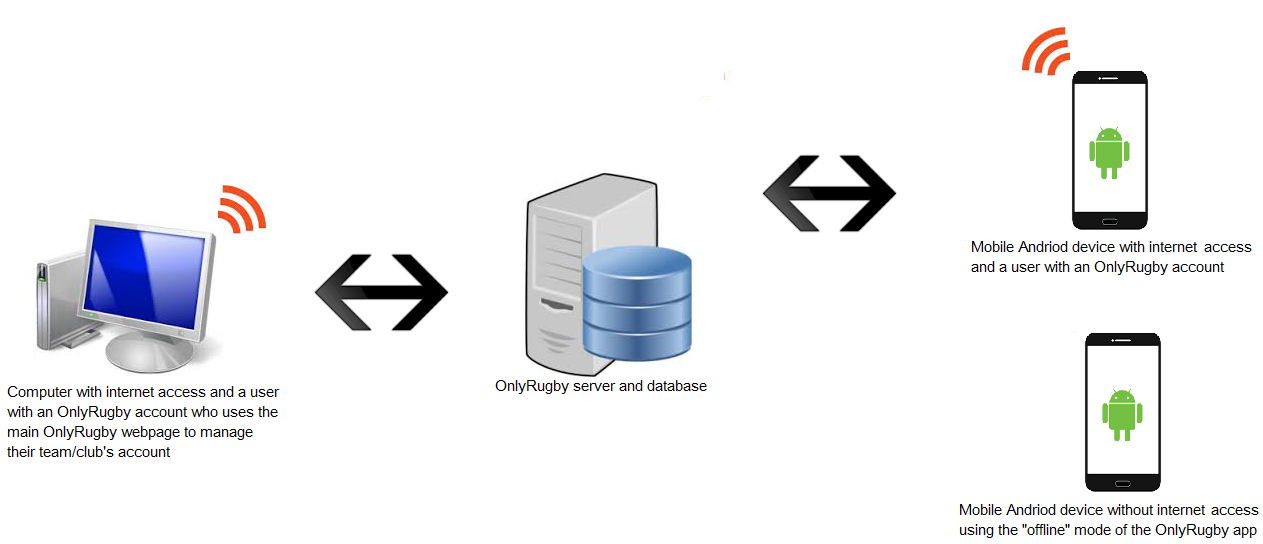
\includegraphics[width=0.9\textwidth] {./images/SystemConfiguration2.png}\\[0.4cm]
\end{center}

\newpage

\section{Installation}
\begin {itemize}
	\item The user must go on GitHub ( \url {https://github.com/hermankeuris/OnlyRugbyApp/tree/master/Install}) and download the application's APK directly (i.e. Only Rugby Score Keeper.apk). You can either download this through your mobile device's web browser directly or first download it on a computer and then copy the APK file to your andriod device through a USB connection with the computer.
	\begin{center}
  		 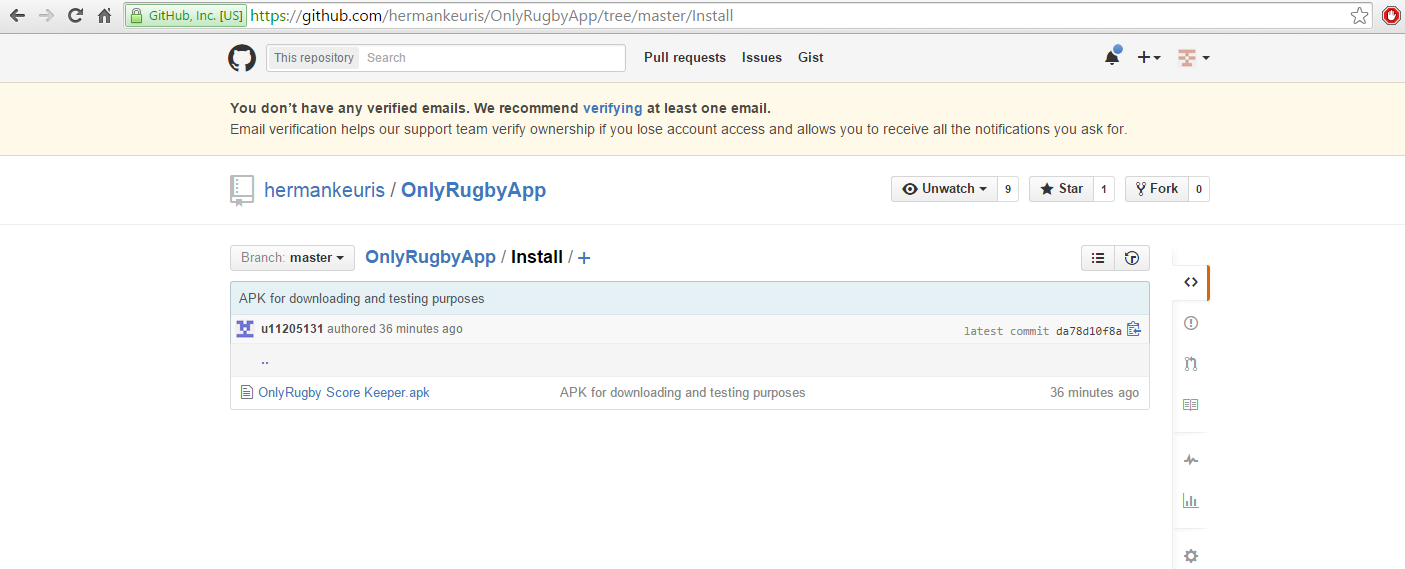
\includegraphics[width=0.9\textwidth] {./images/APKdownload.png}\\[0.4cm]
	\end{center}
	\item To allow your Andriod device to run this APK you will first have to enable your device to allow the installation of files from ''unknown'' sources. This is done by going to your device's Settings \textgreater  Security and checking the ''Unknown Sources'' checkbox.
	\begin{center}
  		 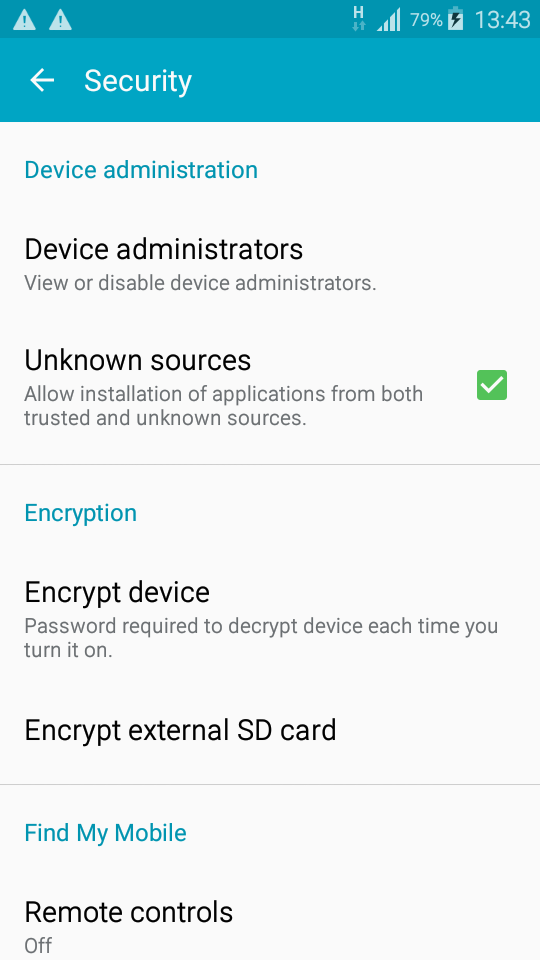
\includegraphics[width=0.4\textwidth] {./images/unknownsources.png}\\[0.4cm]
	\end{center}
	\item In the case of having directly downloaded the APK on your Android device you could then go to the directory where the APK is stored (most likely the ''Downloads'' folder) and click the APK's icon. A pop-up will then appear giving you the option of installing the APK on your device.
	\item In the case of having first downloaded the APK on a computer you should then copy the APK file to some easily accessible directory on the Android device (e.g. ''Downloads'') and then follow the same steps as specified in the previous bullet.
	\begin{center}
  		 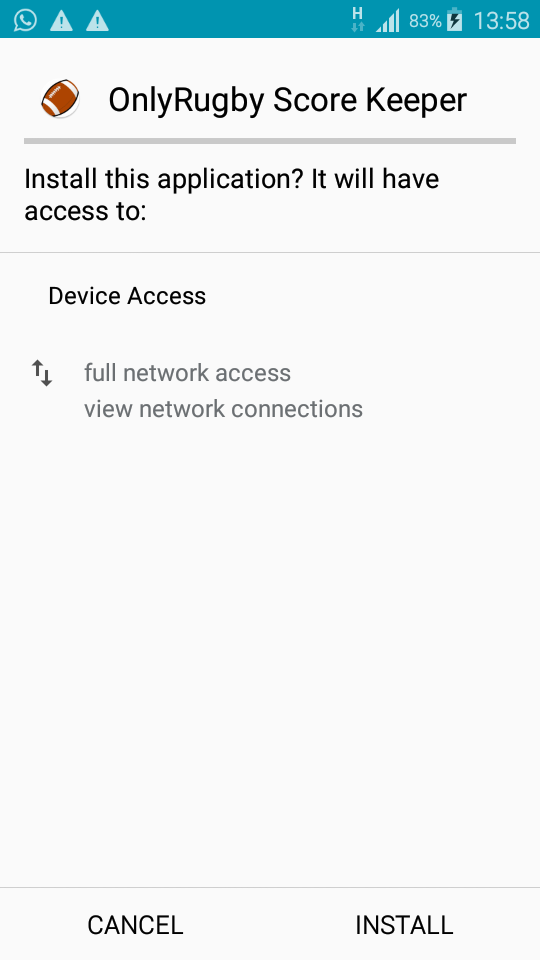
\includegraphics[width=0.4\textwidth] {./images/installation.png}\\[0.4cm]
	\end{center}
	\item To be able to use the application to its full potential the user will have to have both themselves and their club/team registered on the main OnlyRugby website. The user will also have to be registered as having the proper authority to log match information on behalf of his/her club/team. 
\end{itemize}

\newpage

\section{Getting started}
	\begin {itemize}
		\item To get access to use the app, the team you represent should already be registered with the main site.
		\item You also need to have a personal account and your team should have chosen you as their dedicated score keeper.
		\item When all the requirements are satisfied, simply log on to the app with your credentials as you registered them on the website.
		\item You will not be permitted to score a match that is not in the progress of being played.
		\item Once a match is available you can start logging different states of the game, such as tackles, scores, line-outs, substitutions etc.
		\item Once a match is completed, the information can be verified or corrected as needed (such as adding unknown player's names) before being finally submitted to the server for storage in the main database.
		\item Usernames are unique and cannot be changed once you have registered it.
		\item Passwords can be changed using the websites Change Password function in account settings.
		\item Pressing the "back" button on your device twice pops up a notification asking if you really want to exit to prevent accidental app closure. Choosing "Yes" will close the app and all relevant main threads running.
	\end{itemize}

\newpage

\section{Using the system}
The functionality of the app will be spread between the following use cases:

	\subsection{Login/Logout}
		\begin {itemize}
			\item The first screen after choosing "Login" on the main screen, the user will be presented with two fields: One for the username and one for the password. The user enters the requested details and it gets authenticated. Only when the correct information is supplied, will the user be able to continue to the game menu.
			\item The login information will be used to load the next game that needs scoring.
			\item The user gets logged out of the app every time they exit, allowing someone else to be able to log in as well and ensuring security of information.
		\end{itemize}
		
  		\begin{center}
    			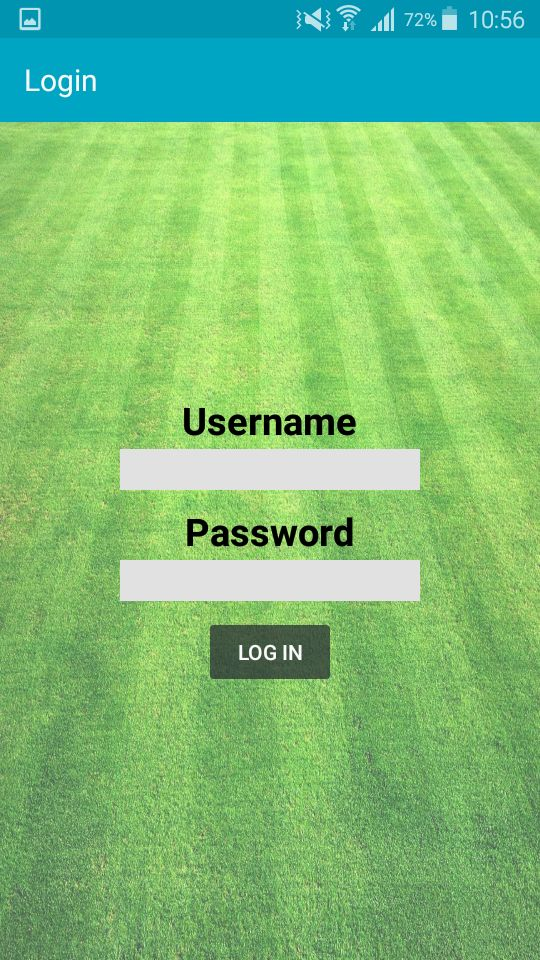
\includegraphics[width=0.4\textwidth]{./images/login_menu.jpg}
  		\end{center}

\newpage		

	\subsection{Load Info}
		This use case pertains to the loading of any and all info you can see and not see in the app itself. A version of it is called by nearly every other function in the app, since it handles all the retrieval from the database via the main server.
		\begin{itemize}
			\item After the user is logged in, information is loaded on what teams the user is allowed to score for. This is done by sending a query with the token (already received when logging in) to the server and retrieving the information associated with this particular user. All of the information is stored on the device's local database for offline usage.
			\item In the event that a match can be scored and the user decides to do so, the data pertaining to that match will be loaded from the device's local database, since it is already stored from the previous request to the server. This will return the names and positions of the players of both teams (if available).
			\item During the match, local storage is implemented to store any data relevant to the match and then uploaded once the app establishes a connection with the server.
		\end{itemize}

\newpage

	\subsection{Game Time}
	This use case is used to log the start and end time of each half of a match, as well as any intervals during which time was lost (the game was paused) and a reason for this time loss (injury, match official consultation, replacement of damaged player clothing). 
	\\ \\
	Usage:
	\begin{itemize}
		\item The game time is displayed at the top of the UI.
		\item The clock is started by tapping the clock. A pop-up will appear with the option, Play. Once it is tapped, the game begins.
		\item When the clock is running, tapping the clock will create a pop-up with 3 options: Pause, Reset and Start Second Half/End Game Clock.
		\item If Pause is selected, the clock will pause and present the user with a pop-up that presents legal reasons for the pause.
		\item If Reset is selected, the clock resets to 0:00 and pauses, allowing the user to restart the current half.
		\item While in the first half, Start Second Half is displayed, which ends the current half and starts the new one.
		\item While in the second half, End Game Clock is displayed, which will stop the clock completely and prevent the user from entering new events.
	\end{itemize}

	\begin{center}
    		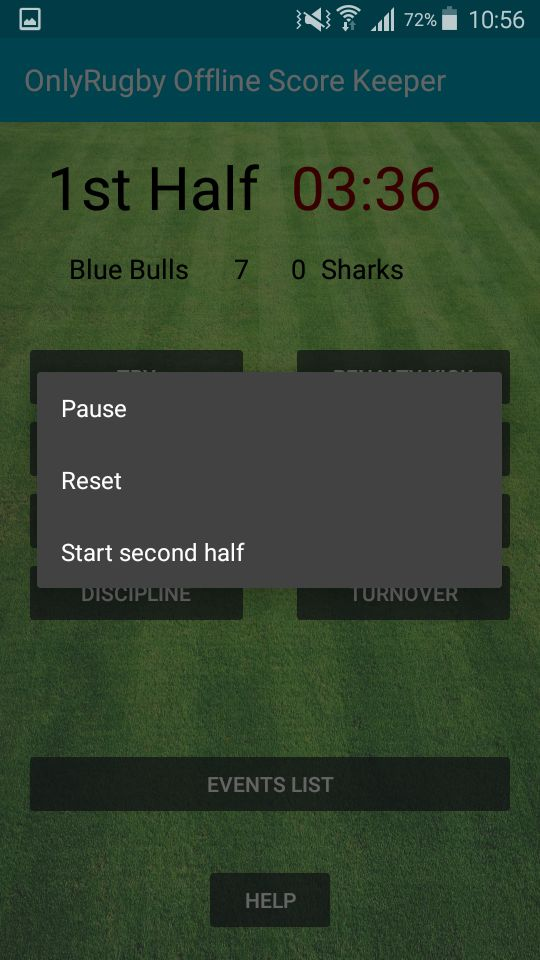
\includegraphics[width=0.4\textwidth]{./images/game_clock.jpg}
  	\end{center}
	
\newpage

	\subsection{Scoring}
		During game time (i.e. while the OnlyRugby app is being used to log the information of a match currently being played ) the Scoring function will be used each time a player from either team scores points for their team (be it through a try, penalty kick, drop-kick or a conversion kick following a try). The Scoring function works as follows:
		\begin{enumerate}
			\item At the main menu for the match logger the user gets to specify what type of score it should log. This page displays buttons titled 'Try', 'Penalty Kick' and  'Drop-kick' (note that 'Conversion Kick' is not an option as it can only be attempted after a successful try). 
		\begin{center}
	 	 	 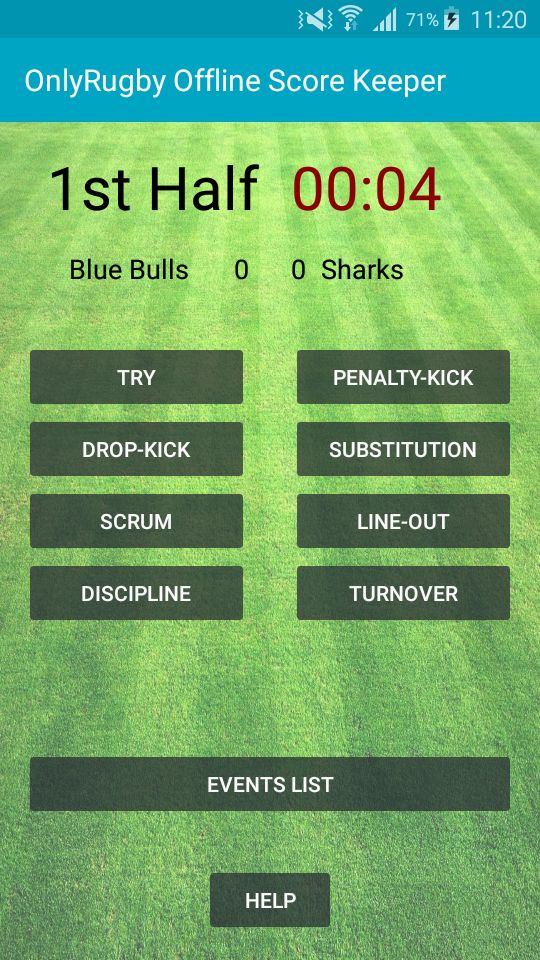
\includegraphics[width=0.4\textwidth] {./images/game_menu.jpg}\\[0.4cm]
		\end{center}
			\item Once the user has selected a score type and pressed the relevant  button to log that type's score information they are redirected to a page which asks them to indicate which team scored by pressing either of two buttons which each have the names of the respective teams on them.
		\begin{center}
  			 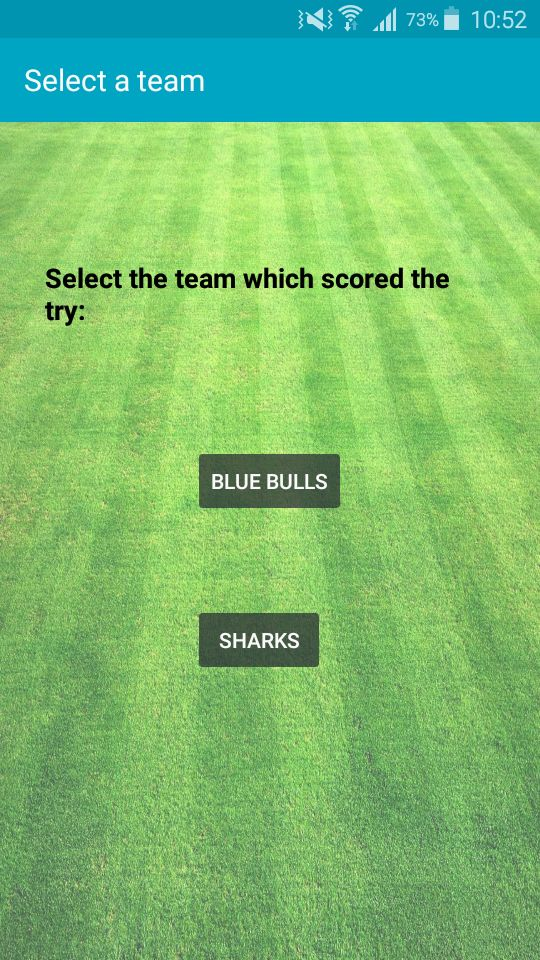
\includegraphics[width=0.4\textwidth] {./images/choose_try_team.jpg}\\[0.4cm]
		\end{center}
			\item The app then redirects the user to another page which has a list of 23 options representing the 15 on-field players and the 7 reserve players of the previously selected team, as well as an 'Unknown' option. (The reason why reserve players are also displayed is in case the user misses logging a substitution, and the list of on-field players is therefore outdated, then they can still select the correct player). Each option has the player's position/jersey number on it as well as the player's name (if that information is provided on the database). This 'Unknown' option is in case the user, for some reason, is not sure who scored on this team. The user is asked to select one of these players/buttons as the player who scored.
		\begin{center}
  			 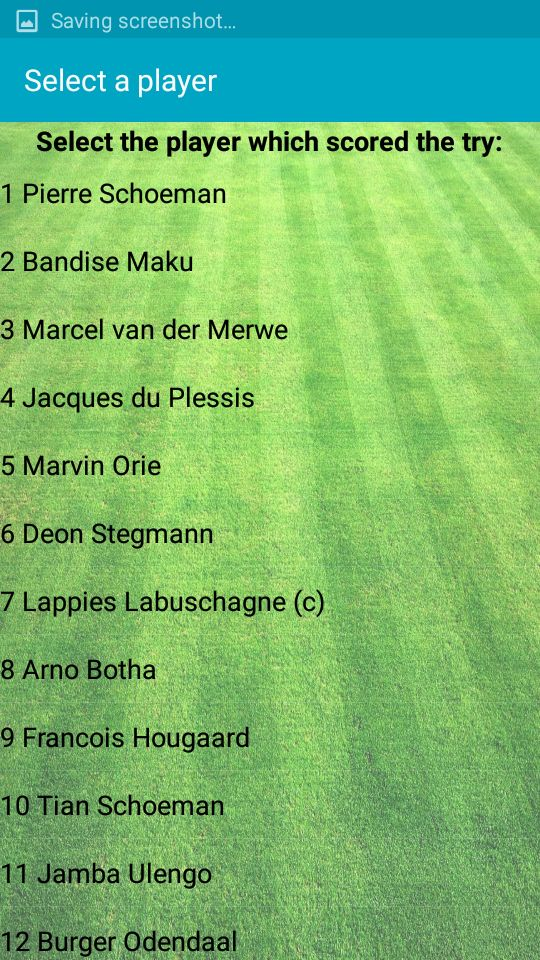
\includegraphics[width=0.4\textwidth] {./images/choose_try_player.jpg}\\[0.4cm]
		\end{center}
			\item In most cases the user is then done entering the score information but in the case of a 'Try' more steps must be completed:
				\begin{itemize}
					\item The user is once again shown the 'player selection page' but is this time asked to select the player who attempted the conversion kick.
					\item Once a player has been selected a small pop-up message is displayed asking the user whether the conversion attempt was successful with options to select either 'Yes' or 'No'.
				\begin{center}
  					 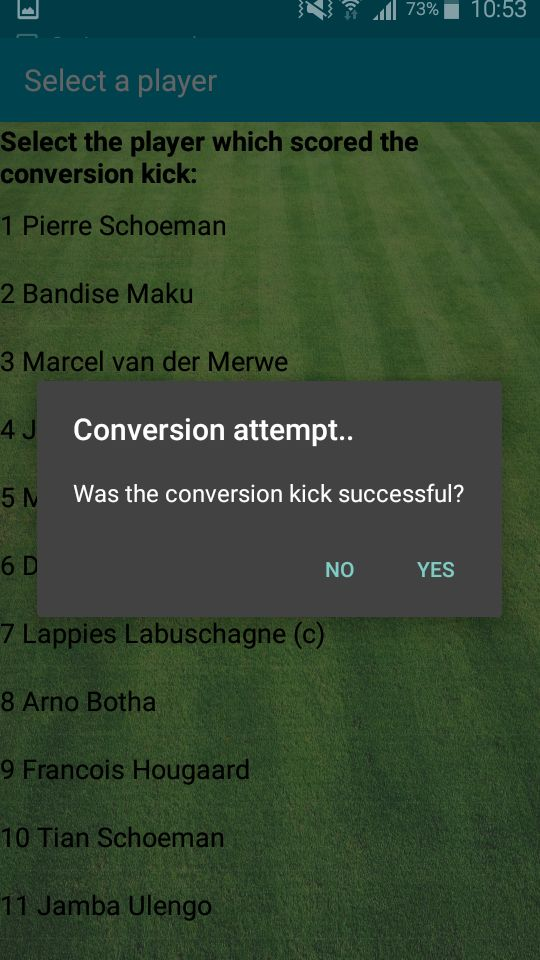
\includegraphics[width=0.4\textwidth] {./images/try_converted.jpg}\\[0.4cm]
				\end{center}
				\end{itemize}
		\item After a score has been logged the user is returned to the main match logger menu and the relevant team's score is updated.
		\begin{center}
  			 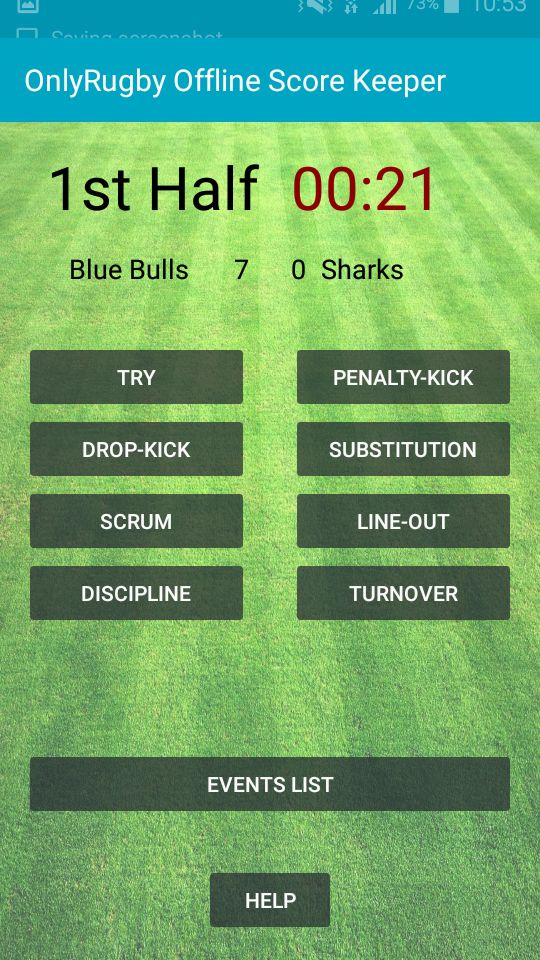
\includegraphics[width=0.4\textwidth] {./images/score_increased.jpg}\\[0.4cm]
		\end{center}
		\end{enumerate}
	On all of the above described pages the user also has the option of using the phone's  'Back' button which redirects the user to the previous page.

	\subsection{Substitutions}
		During game time the Substitutions function will be used to log any changes made to both the on- and off-field players (i.e. reserve players) of either team. This function will work as follows:
		\begin{enumerate}
			\item Once the player has pressed the button to log player substitutions they are redirected to a page which asks them to indicate which team is substituting a player by pressing either of two buttons which each have the names of the respective teams on them.
			\begin{center}
  				 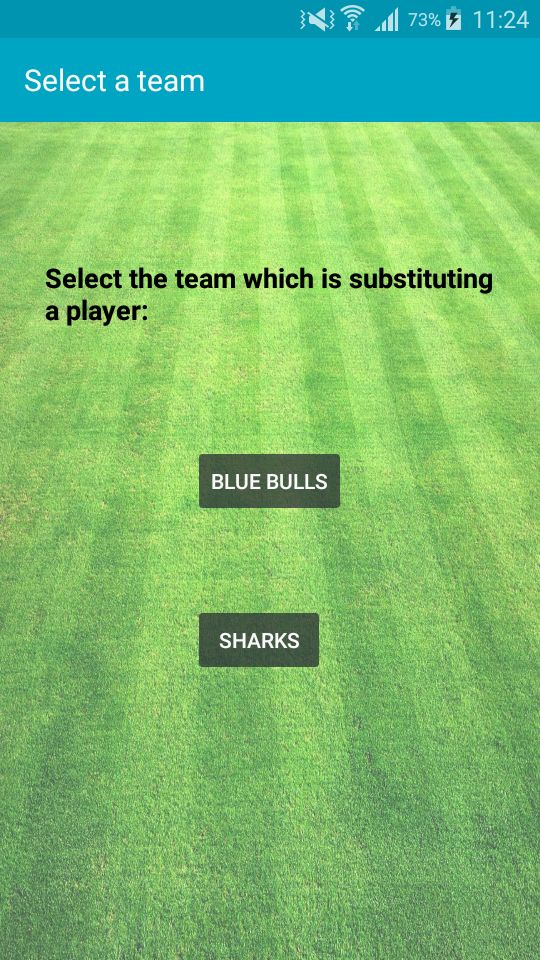
\includegraphics[width=0.4\textwidth] {./images/choose_substitute.jpg}\\[0.4cm]
			\end{center}
			\item The app then redirects the user to the 'player selection page' (as described in the Scoring section) which comprises of 23 options representing the on-field- and reserve players of the selected team, as well as the 'Unknown' option.
			\begin{center}
  				 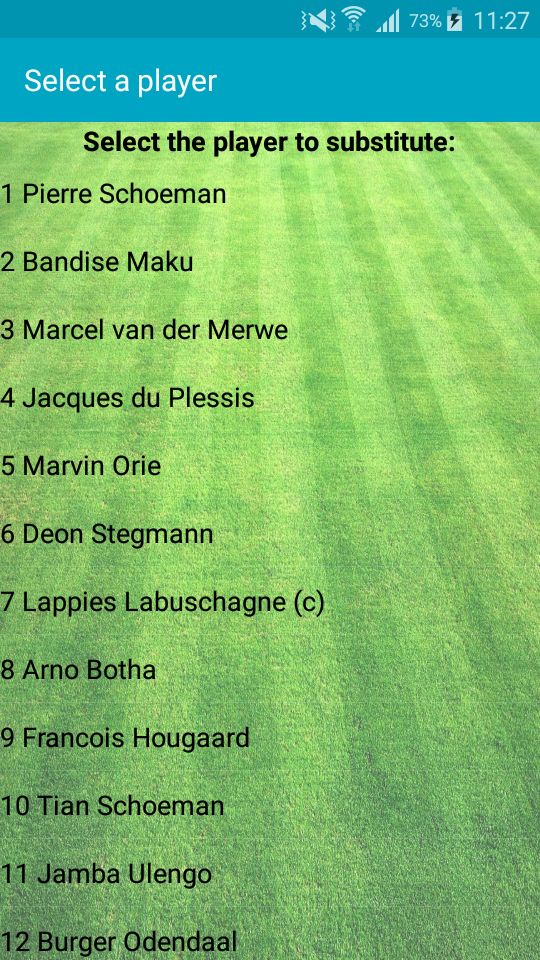
\includegraphics[width=0.4\textwidth] {./images/choose_substitute_player.jpg}\\[0.4cm]
			\end{center}
			\item The app then redirects the user to the same 'player select' page but with a new heading asking the user to select a reserve player to swap out with the previously selected on-field player. This information is then logged in the Events List. If there is not a full reserve team of 7 players stored on the server's database then the remaining players required to form a team of 7 are substituted with distinct 'Unknown' players to hold place for any players which might function as reserve players during match time but who were not logged on the main site's database (which means the app therefore does not have information about them).

	On all of the above described pages the user also has the option of using the phone's  'Back' button which redirects the user to the previous page and ignores the information that was logged on the page it is now leaving.
		\end{enumerate}

\newpage

	\subsection{Discipline}
		During game time (i.e. while the OnlyRugby app is being used to log the information of a match currently being played ) the Discipline function will be used each time a player performs an infraction that causes them to receive a card. The Discipline function works as follows:
		\begin{enumerate}
			\item Once the user has pressed the button to log the disciplinary action's information they are redirected to a page which asks them to indicate which team's player was given a card, by pressing either of two buttons which each have the names of the respective teams on them.
			\item The app then redirects the user to the 'select user' page which has the 22 on- and off-field players. Each option has the player's position/jersey number on it as well as the player's name (if that information is provided on the database). This page also has an 'Unknown' option in case the user, for some reason, is not sure who the player being disciplined is. The user is asked to select one of these players as the player who was disciplined.
			\item The app then redirects the user to another page which has 2 buttons, to indicate if a yellow or red card was given.
		\end{enumerate}

	\begin{center}
  		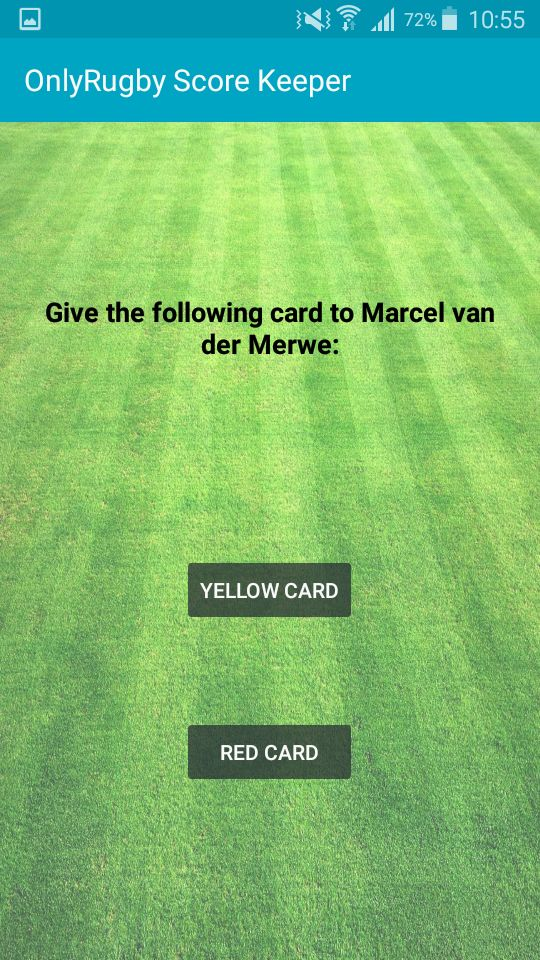
\includegraphics[width=0.4\textwidth] {./images/choose_card.jpg}\\[0.4cm]
	\end{center}

	Player's with cards then have their information displayed with a coloured background (yellow for a yellow card, red for a red card) for the rest of the match (or in the case of a yellow card until the user revokes the card). These players are no longer selectable when using any of the scoring functions (i.e. a punished player cannot be on the field and can therefore not score).

	\begin{center}
  		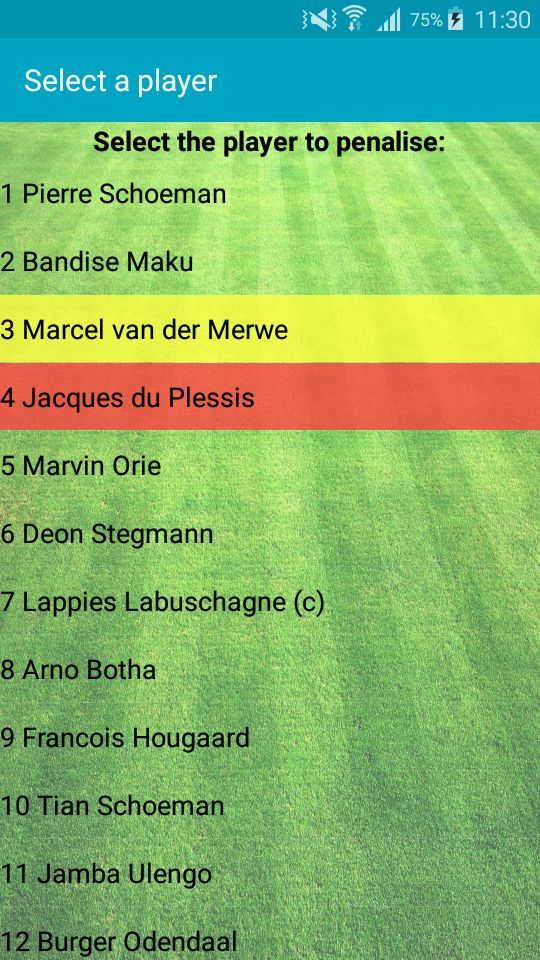
\includegraphics[width=0.4\textwidth] {./images/discipline_display.jpg}\\[0.4cm]
	\end{center}

	To remove a player's yellow card:
	\begin{itemize}
		\item Use the Discipline function again and select the player with the yellow card.
		\item A small pop-up menu will appear asking the user if they want to remove that player's card with the options of 'Yes' and 'No'.

		\begin{center}
  			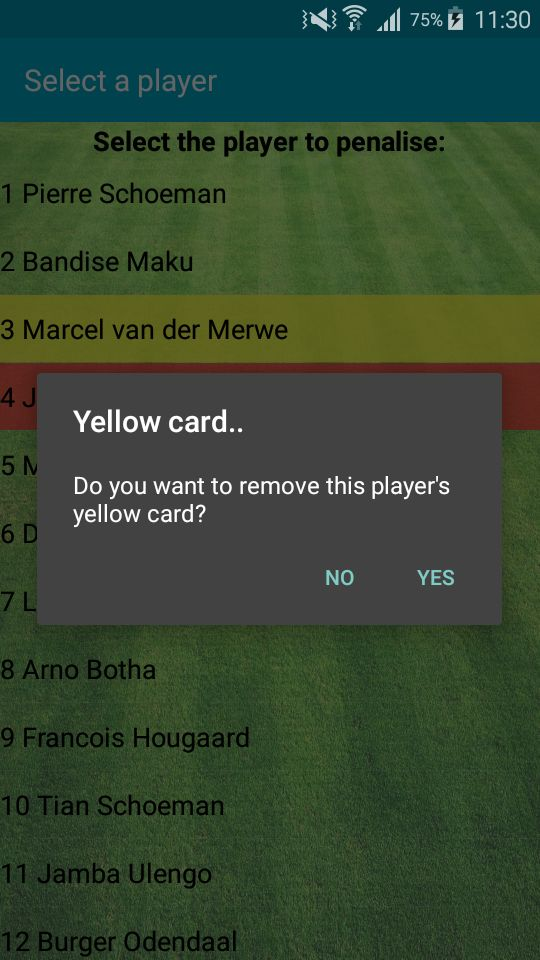
\includegraphics[width=0.4\textwidth] {./images/remove_discipline.jpg}\\[0.4cm]
		\end{center}

		\item Once the yellow card has been removed the player can then be logged in Scoring functions.
	\end{itemize}

	On all of the above described pages the user also has the option of using the phone's  'Back' button which redirects the user to the previous page and ignores the information that was logged on the page it is now leaving.

\newpage

	\subsection{Line-outs}
	During game time the Line-outs function will be used to log when the ball has gone out of the field of play and a line-out has occurred. The team that manages to take possession of the ball during the line-out is the winner. This function will work as follows:
	\begin{itemize}
		\item Once the user has pressed the button to log the line-out's information they are redirected to a page which asks them to indicate which team won the line-out by pressing either of two buttons which each have the names of the respective teams on them.
	\end{itemize}

	\begin{center}
  		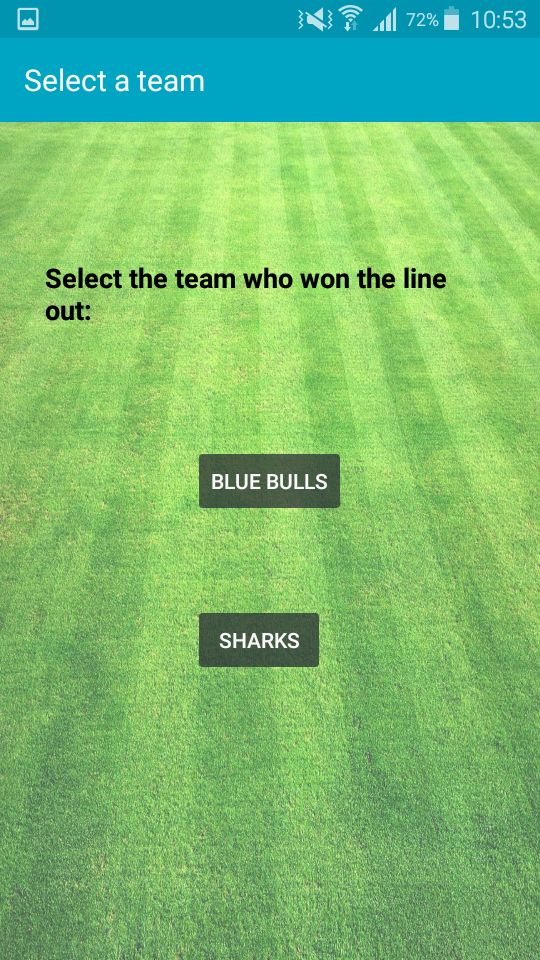
\includegraphics[width=0.4\textwidth] {./images/choose_lineout.jpg}\\[0.4cm]
	\end{center}

	On all of the above described pages the user also has the option of using the phone's  'Back' button which redirects the user to the previous page and ignores the information that was logged on the page it is now leaving.

\newpage

	\subsection{Scrums}
		During game time (i.e. while the OnlyRugby app is being used to log the information of a match currently being played ) the Scrum function will be used each time a scrum is initiated on field.  The Scrum function works as follows:
		\begin{itemize}
			\item Once the user has pressed the button to log the scrum's information they are redirected to a page which asks them to indicate which
			team won the scrum by pressing either of two buttons which each have the names of the respective teams on them.
		\end{itemize}

		\begin{center}
  			 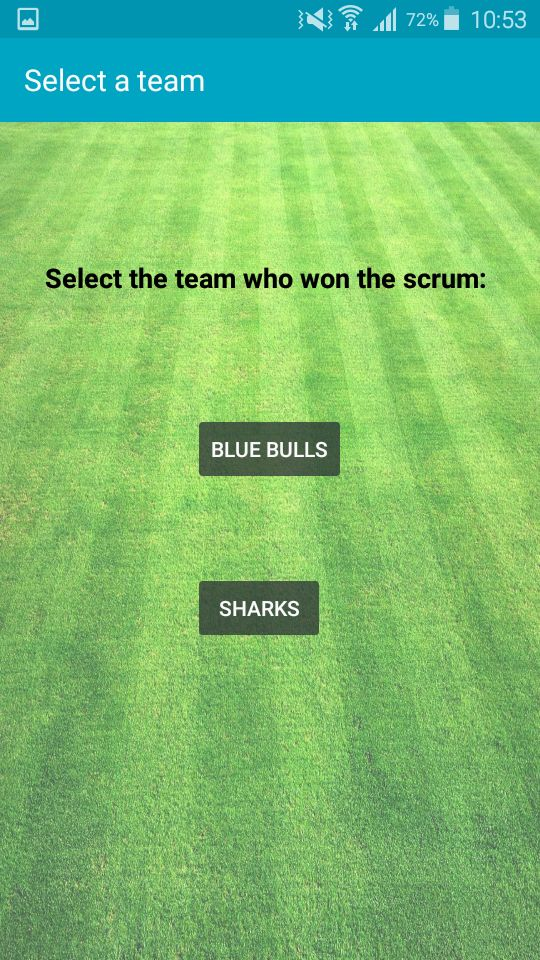
\includegraphics[width=0.4\textwidth] {./images/choose_scrum_team.jpg}\\[0.4cm]
		\end{center}

	On all of the above described pages the user also has the option of using the phone's  'Back' button which redirects the user to the previous page and ignores the information that was logged on the page it is now leaving.

\newpage

	\subsection{ Turnovers}
		During game time (i.e. while the OnlyRugby app is being used to log the information of a match currently being played ) the Turnover function will be used each time a player from either team manages to take possession of the ball from an opposing player. The Turnover function works as follows:
		\begin{itemize}
			\item Once the user has pressed the button to log the turnover's information they are redirected to a page which asks them to indicate which team won the turnover by pressing either of two buttons which each have the names of the respective teams on them.
			\item The app then logs the occurrence of the turnover as well as the possession of the ball.
		\end{itemize}

		\begin{center}
  			 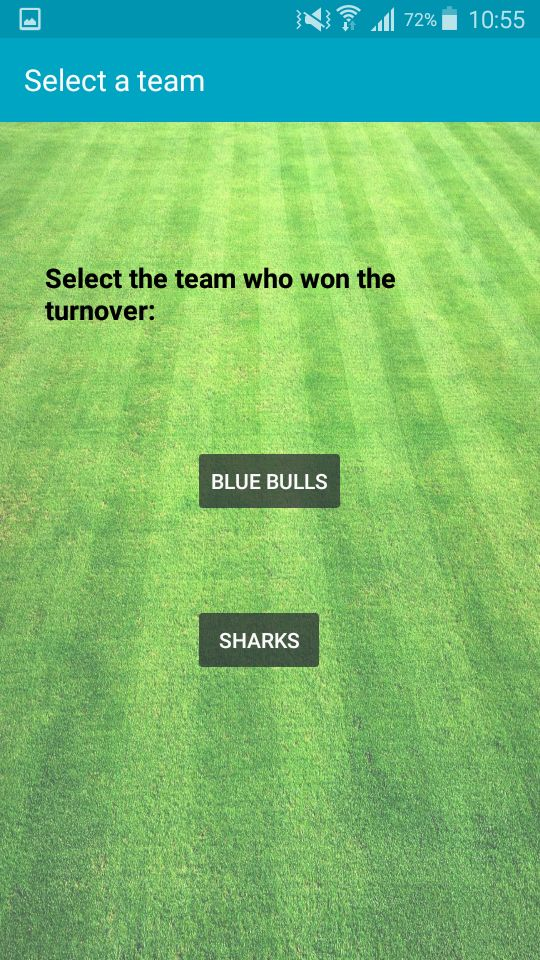
\includegraphics[width=0.4\textwidth] {./images/choose_turnover.jpg}\\[0.4cm]
		\end{center}

	On all of the above described pages the user also has the option of using the phone's  'Back' button which redirects the user to the previous page and ignores the information that was logged on the page it is now leaving.

\newpage

\subsection{ Events List}
		During game time (i.e. while the OnlyRugby app is being used to log the information of a match currently being played ) the Events List functionality will be used each time an event is logged (such as Tries and when the second half begins). The Events List functionality works as follows:
		\begin{enumerate}
			\item Once the user has pressed the button to view the list of events, they are redirected to a page that contains a chronological (sorted by each event's timestamp) of all the events and a button to add a new event.

			\begin{center}
  				 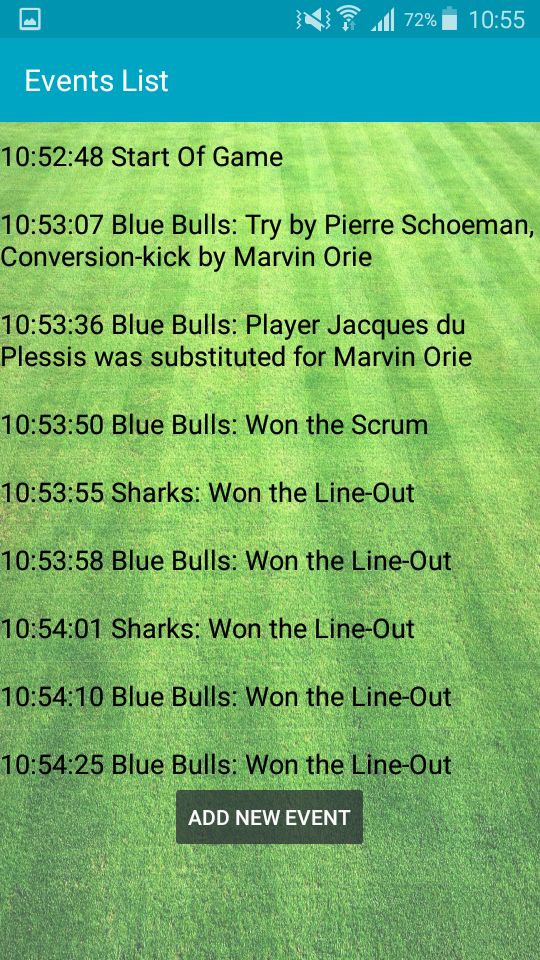
\includegraphics[width=0.4\textwidth] {./images/eventslist.jpg}\\[0.4cm]
			\end{center}

			\item By pressing on an event, the user is redirected to a page that contains 2 buttons: Alter Event and Delete Event.

			\begin{center}
  				 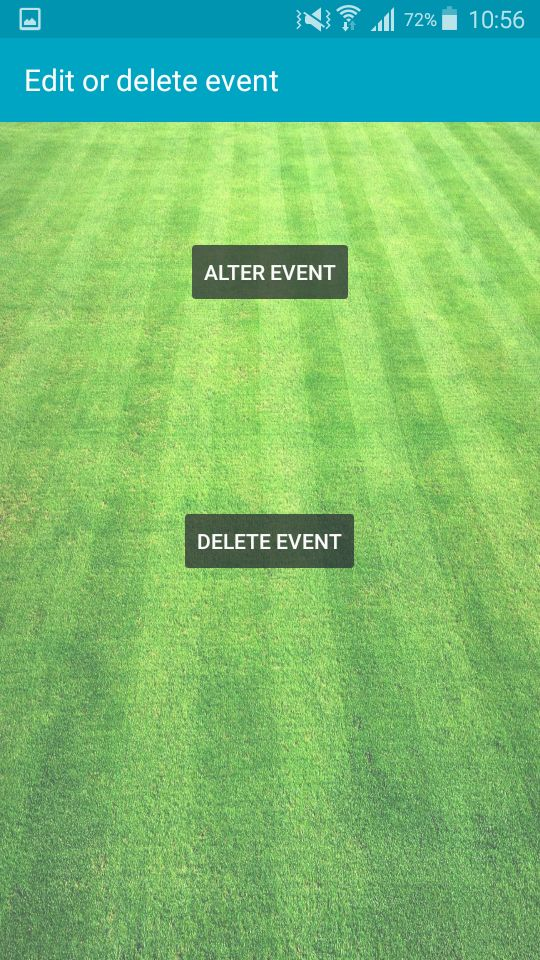
\includegraphics[width=0.4\textwidth] {./images/alter_and_delete.jpg}\\[0.4cm]
			\end{center}

				\begin{enumerate}
					\item Alter Event follows the same steps that were used when the event was created, but replaces the event at the selected index and makes use of its timestamp. All the changes that the replaced event made are reversed and the new events changes are implemented.
					\item Delete Event creates a pop-up window that asks the user if they wish to delete the event. If they select no, no changes are made. If the user selects yes, the event is removed from the list and the changes that it made are reversed.

					\begin{center}
  						 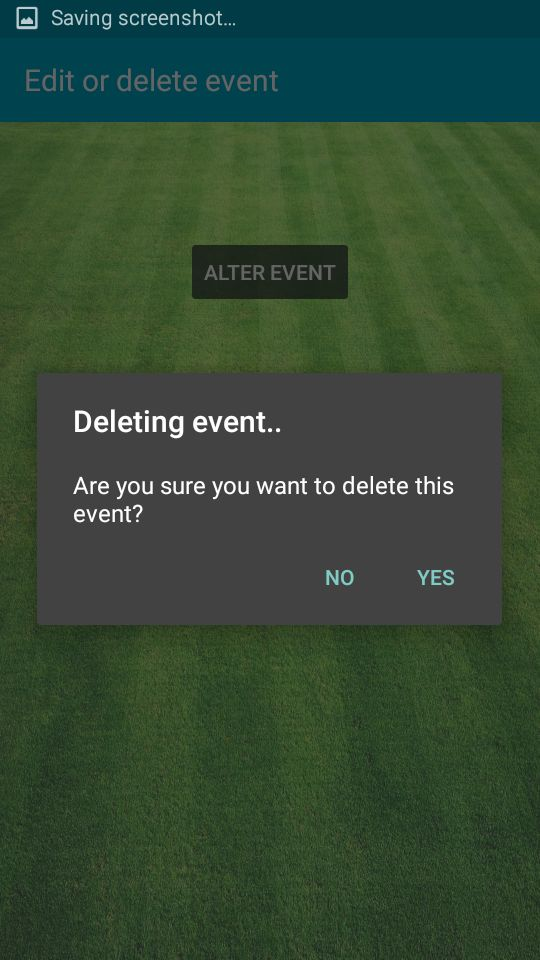
\includegraphics[width=0.4\textwidth] {./images/delete_event.jpg}\\[0.4cm]
					\end{center}

				\end{enumerate}

		\item By pressing the create event button, the user is redirected to a page that contains an input box that allows for a custom timestamp to be entered. If the timestamp is in the wrong format or it occurs before the game starts, the current time is used. The user can then select which event occurred and follows the normal procedure for that event. In this way, if an event was missed, it can be added later.

		\end{enumerate}

	On all of the above described pages the user also has the option of using the phone's  'Back' button which redirects the user to the previous page and ignores the information that was logged on the page it is now leaving.

\section{Troubleshooting}
	In the event that the app crashes or something goes wrong, a comprehensive error message will be provided to the user with an error code. This error code can then be used with the built-in troubleshooting guide for a more descriptive explanation of the error. Additionally, an error log file will also be created, containing all the relevant information pertaining to the crash.
		
\end{document}
